% Copyright 2018-2020 Melvin Eloy Irizarry-Gelpí
% \setcounter{chapter}{4}
\chapter{Newton's Third Law}
%
In this experiment you will check the validity of Newton's third law of motion.
%
\section{Preliminary}
%
The \textbf{third law of motion} can be stated as follows:
\begin{itemize}
    \item Whenever A exerts a force $\vec{F}_{AB}$ on B, B exerts a force $\vec{F}_{BA}$ on A.
    \item The \textbf{magnitude} of the forces $\vec{F}_{BA}$ and $\vec{F}_{AB}$ are equal.
    \item The \textbf{direction} of the force $\vec{F}_{BA}$ is the exact opposite of the direction of the force $\vec{F}_{AB}$.
\end{itemize}
In more mathematical terms,
\begin{align}
    \vert \vec{F}_{BA} \vert &= \vert \vec{F}_{AB} \vert & \vec{F}_{BA} &= - \vec{F}_{AB}
\end{align}
One way to test the third law would be to measure the force acting on two bodies and verify that the magnitudes are the same, but that the directions are opposite.

There is a \textbf{common misconception} about the third law. Sometimes, it is stated as
\begin{itemize}
    \item For every action, there is an equal and opposite \textbf{reaction}.
\end{itemize}
This wording leads to an \textbf{incorrect} picture because it introduces an order in time, as in object A first acts on object B, and then, as a reaction, object B acts on object A. This is \textbf{incorrect}. Both forces in Newton's third law appear \textbf{at the same time}. You can check this by measuring the force across time. If the reaction picture were accurate, then you would see a time-delay in one of the forces. Another way to state this is that there is a symmetry between the objects in the sense that there is no breakdown into aggressor and receiver.
%
\section{Experiment}
%
You used two force sensors to measure the amount of force acting on each other. For definiteness, the sensor on the left is called ``Sensor L'', and the sensor on the right is called ``Sensor R'' To check different aspects of the third law, you performed three kinds of experiments:
\begin{itemize}
    \item Sensor L pulls/pushes on sensor R.
    \item Sensor R pulls/pushes on sensor L.
    \item Both sensors pull/push on each other.
\end{itemize}
Furthermore, you tried different attachments on the force sensors:
\begin{itemize}
    \item String (pulling)
    \item Elastic Band (pulling)
    \item Bumpers (pushing)
    \item Magnets (pushing)
\end{itemize}
The force sensors give you force values (in N) over time (in s).
%
\section{Analysis}
%
Here is what to do. For illustration purposes, I will work with the runs using the \textbf{magnets}.
%
\subsection{Plot Both Forces Versus Time}
%
With the force values from each sensor you can make line charts. Figures \ref{figure:05.ff.L}, \ref{figure:05.ff.R}, and \ref{figure:05.ff.B} display the three runs with magnets. As you can see, the three charts are very symmetric about the horizontal axis, supporting the notion that each force sensor measures about the same amount of force at the same amount of time, but with different signs.

Another thing to notice, is that the three charts mentioned above are very similar and without any labels one could not tell if either sensor is doing the pushing, or both. For example, there is nothing special about Figure \ref{figure:05.ff.L} that distinctively indicates that the left sensor is pushing on the right sensor.
%
\subsection{Plot Sum of Forces Versus Time}
%
Besides visually examining the charts with the two force columns, you can calculate and also visualize the \textbf{sum of the two force columns}. Figures \ref{figure:05.sf.L}, \ref{figure:05.sf.R}, and \ref{figure:05.sf.B} display the three runs with magnets. As you can see the sum of the forces takes on very small values with no clear pattern. Indeed, the values are comparable to the starting values before any pushing is done. This indicates that, for practical purposes, the sum of the two forces amounts to noise. That is, the result of adding the two force columns gives a column of force values that are indistinguishable from a noise reading.

Again, all three charts here are very similar, so without labels you could not tell which chart corresponds to which run (i.e. which sensor was doing the pushing).
%
\subsection{Find Time-Averaged Values}
%
In order to summarize each run, you can calculate the time-averaged value of the amount of force acting on each sensor, and also the time-averaged value of the sum of the forces. In Table \ref{table:05.results} you can find my results. As you can see, the magnitude of the values in the second column are very close to the magnitude of the values in the third column. This is consistent with Newton's third law. Also, the values in the fourth column are very small. Although the values in the fourth column are not exactly zero, the values are indistinguishable from noise values. This observation allows me to conclude that the sum of forces averages to a value that could be measured as effectively zero. This is also consistent with Newton's third law.

Another observation from Table \ref{table:05.results} is that there is no clear pattern among the runs associated to a given attachment. That is, from the values alone, you cannot tell which sensor is pushing/pulling.

Yet another observation from Table \ref{table:05.results} is that both pulling cases are consistent, and also both pushing cases are consistent. That is, you cannot tell from the values which run had a string or an elastic band. This is as expected: Newton's third law of motion does not depend on the nature of the force.
%
\section{My Data}
%
Here is a breakdown of my runs:
\begin{enumerate}
    \item String (left pulling)
    \item String (right pulling)
    \item String (both pulling)
    \item String (left pulling)
    \item String (right pulling)
    \item String (both pulling)
    \item Elastic band (left pulling)
    \item Elastic band (right pulling)
    \item Elastic band (both pulling)
    \item Bumpers (left pushing)
    \item Bumpers (right pushing)
    \item Bumpers (both pushing)
    \item Magnets (left pushing)
    \item Magnets (right pushing)
    \item Magnets (both pushing)
\end{enumerate}
I got distracted and accidentally forgot to replace the string with the elastic band, so collected double the amount of data for the string.
%
\section{Your Data}
%
You should have three runs of data for each of the four attachments for the force sensor (total number of runs should be twelve). For each run, you should have a time column, and two force columns. 
%
\newpage
\section{Your Laboratory Report}
%
Your laboratory report should include the following:
\begin{enumerate}
    \item Choose \textbf{one} of the four attachments (string or elastic band or bumpers or magnets). For that choice, make the following \textbf{line charts}:
    \begin{enumerate}
        \item Three charts like Figure \ref{figure:05.ff.L} (one chart for each of the three runs) with force in the vertical axis and time in the horizontal axis, showing \textbf{both} force columns.
        \item Three charts like Figure \ref{figure:05.sf.L} (one chart for each of the three runs) with force in the vertical axis and time in the horizontal axis, showing the \textbf{sum of forces}.
    \end{enumerate}
    \item A table like Table \ref{table:05.results} with the time-averaged values for the force on L, force on R, and sum of forces, for \textbf{all twelve} runs.
\end{enumerate}
You should also include answers to the following questions:
\begin{enumerate}
    \item Looking at your table of time-averaged values (e.g. \ref{table:05.results}), is there a clear pattern that allows you to distinguish runs by the kind of attachment used?
    \item Looking at your table of time-averaged values (e.g. \ref{table:05.results}), is there a clear pattern that allows you to tell from the values which sensor was pushing/pulling?
    \item Besides the sign in the force values, is there are anyway of telling the pushing forces apart from the pulling forces?
    \item Imagine Figures \ref{figure:05.ff.L}, \ref{figure:05.ff.R}, and \ref{figure:05.ff.B} had no labels. Could you tell from looking at a chart whether the left sensor was pushing or the right sensor was pushing or both were pushing?
    \item Imagine Figures \ref{figure:05.sf.L}, \ref{figure:05.sf.R}, and \ref{figure:05.sf.B} had no labels. Could you tell from looking at a chart whether the left sensor was pushing or the right sensor was pushing or both were pushing?
    \item Do you find that Newton's third law holds? Remember that small force values could be indistinguishable from noise.
\end{enumerate}
%
\newpage
\section{Tables}
%
\vspace{\stretch{1}}
\begin{table}[ht]
    \centering
    \begin{tabular}{|l|r|r|r|c|}
        \hline
        Run & Force on L (N) & Force on R (N) & Sum of Forces (N) & Attachment \\
        \hline
        1 & 3.980 & \textminus 4.053 & \textminus 0.073 & \\
        2 & 1.499 & \textminus 1.571 & \textminus 0.071 & String \\
        3 & 1.948 & \textminus 1.976 & \textminus 0.028 & \\
        \hline
        4 & 2.167 & \textminus 2.225 & \textminus 0.058 & \\
        5 & 2.248 & \textminus 2.335 & \textminus 0.086 & String \\
        6 & 3.653 & \textminus 3.771 & \textminus 0.119 & \\
        \hline
        7 & 1.673 & \textminus 1.772 & \textminus 0.098 & \\
        8 & 2.002 & \textminus 2.049 & \textminus 0.047 & Elastic Band \\
        9 & 2.362 & \textminus 2.420 & \textminus 0.059 & \\
        \hline
        10 & \textminus 3.913 & 3.945 & 0.033 & \\
        11 & \textminus 3.670 & 3.692 & 0.022 & Bumpers \\
        12 & \textminus 4.638 & 4.627 & \textminus 0.012 & \\
        \hline
        13 & \textminus 2.121 & 2.089 & \textminus 0.032 & \\
        14 & \textminus 3.008 & 2.968 & \textminus 0.040 & Magnets \\
        15 & \textminus 4.064 & 4.025 & \textminus 0.039 & \\
        \hline
    \end{tabular}
    \caption{Time-Averaged Values.}
    \label{table:05.results}
\end{table}
\vspace{\stretch{1}}
%
\FloatBarrier
\newpage
\section{Figures}
%
\vspace{\stretch{1}}
\begin{figure}[ht]
    \centering
    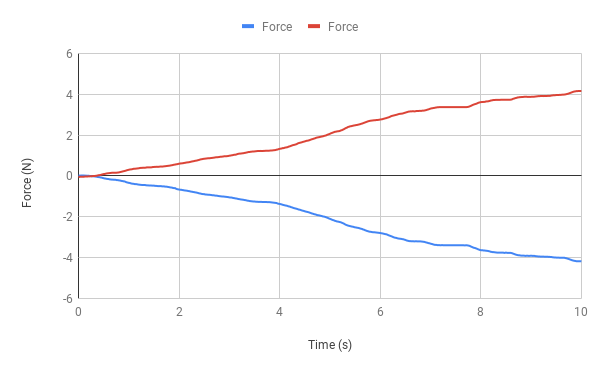
\includegraphics[scale=0.71]{image/05-third-law/Run-13-Both.png}
    \caption{Both Forces versus Time; Left Pushing}
    \label{figure:05.ff.L}
\end{figure}
\vspace{\stretch{1}}
%
\begin{figure}[ht]
    \centering
    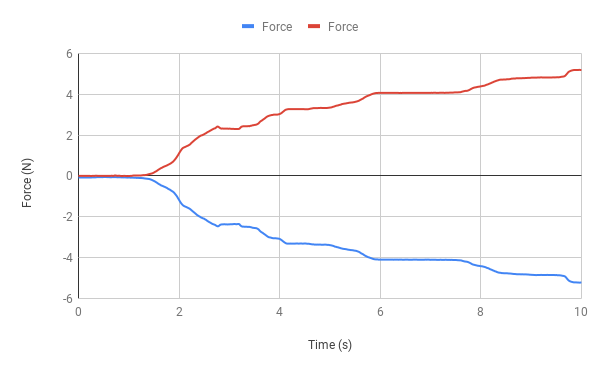
\includegraphics[scale=0.71]{image/05-third-law/Run-14-Both.png}
    \caption{Both Forces versus Time; Right Pushing}
    \label{figure:05.ff.R}
\end{figure}
%
\begin{figure}[ht]
    \centering
    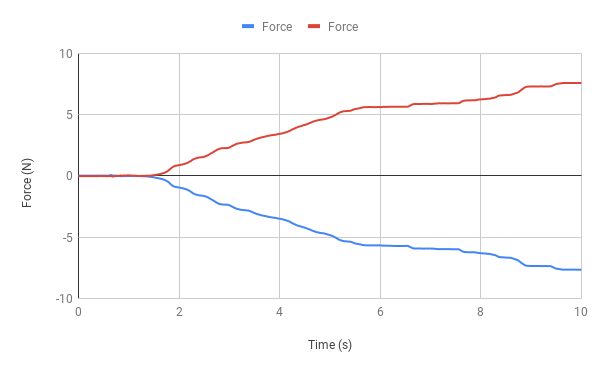
\includegraphics[scale=0.71]{image/05-third-law/Run-15-Both.png}
    \caption{Both Forces versus Time; Both Pushing}
    \label{figure:05.ff.B}
\end{figure}
%
\begin{figure}[ht]
    \centering
    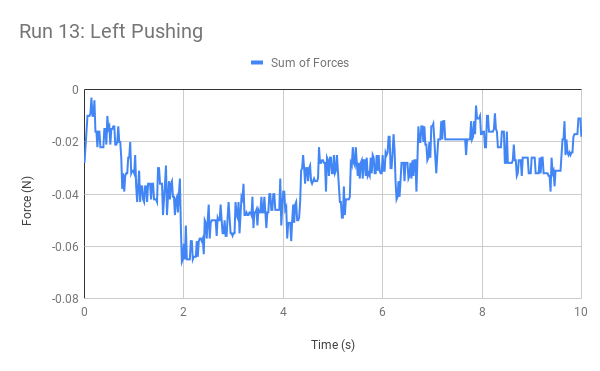
\includegraphics[scale=0.71]{image/05-third-law/Run-13-Left-Pushing.png}
    \caption{Sum of Forces versus Time; Left Pushing}
    \label{figure:05.sf.L}
\end{figure}
%
\begin{figure}[ht]
    \centering
    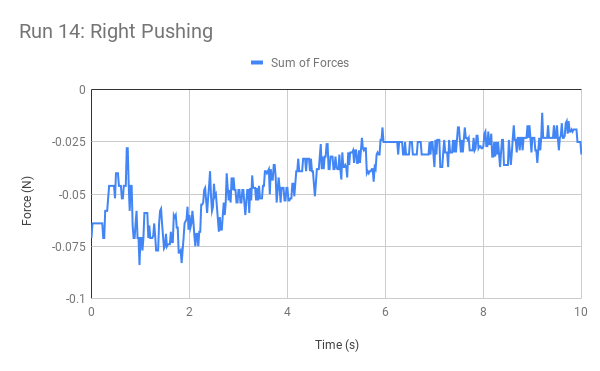
\includegraphics[scale=0.71]{image/05-third-law/Run-14-Right-Pushing.png}
    \caption{Sum of Forces versus Time; Right Pushing}
    \label{figure:05.sf.R}
\end{figure}
%
\begin{figure}[ht]
    \centering
    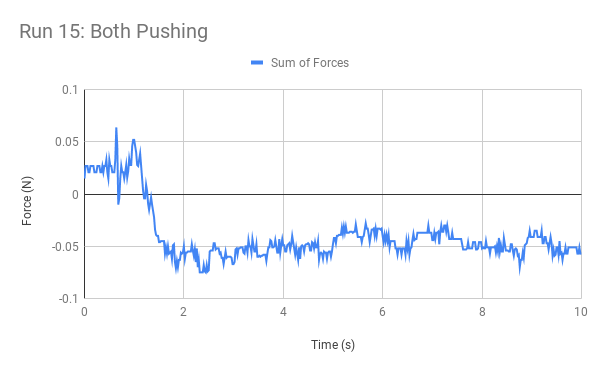
\includegraphics[scale=0.71]{image/05-third-law/Run-15-Both-Pushing.png}
    \caption{Sum of Forces versus Time; Both Pushing}
    \label{figure:05.sf.B}
\end{figure}
%